\section{Pažite technológie}

Našou úlohou v~tejto bakalárskej práci je naprogramovať a~otestovať nami vytvorený ovládač pre mobilného robota. Tento ovládač
bude vytvorený v~jazyku C++ v~systéme ROS. Pred tým ako začneme preberať tento spomenutý ovládač a~robota, ktorého budeme riadiť,
tak~si predstavíme technológie, ktoré budeme používať pri~vytváraní ovládača. Si to Linux, C++, ROS a~samotný robot.

\subsection{Operačný systém}

Na~začiatku našej práce sme sa museli rozhodnúť, či budeme písať program na~náš ovládač v~operačnom systéme Windows 11 alebo
v~operačnom systéme Ubuntu 22.04, ktorý je založený na~Linuxe. Ako programátori sme už dlhšie pracovali s operačným systémom
Ubuntu a~poznáme aj jeho výhody a~nevýhody. To iste platí aj pre operačný systém Windows. Toto sú fakty, ktoré sme zvažovali
pri~výbere operačného systému, ktorý sme používali počas celej bakalárskej práce.

\subsubsection{Windows}

Windows je najpoužívanejším operačným systémom na~počítače na~svete. Je to hlavne preto, že~je jednoduchý na~použivanie
pre netechnických užívateľov. Windows ale nie je bezpečným operačným systémom a~taktiež aj jeho stabilita a~rýchlosť
nie sú na~najvyššej úrovni. Tento operačný systém pozývajú lúdia hlavne na~voľnočasové aktivity ako je hranie hier
alebo v~práci ako napríklad v~kanceláriách na~úpravu tabuliek. Pre nás ako programátorov tento operačný systém nie je
výhodný. Nastavovanie prostredia pre programovanie je v~tomto operačnom systéme oveľa náročnejšie ako v~Linuxe. Podpora
prekladačov programov (z~anglického compiler) je v~tomto operačnom systéme oveľa horšia ako už v~spomenutom Linuxe.

\subsubsection{Ubuntu}

Ubuntu je stabilný a~bezpečný operačný systém, ktorý je založený na~Linuxe. Väčšina ľudí hovori o Linuxe ako o operačnom systéme. Pravdou
to ale nie je. Linux je totižto len \textbf{kernel} (jadro) operačného systému. Kernel je hlavný program, ktorý sa stará o správu hardvéru,
riadenie procesov a~spravu pamäte. Zároveň poskytuje možnosť operačnému systému komunikovať s hardvérom a~poskytuje jednotným programom
prístup k~hardvéru a~jeho častiam.

Linux je používaný skoro vo~všetkých mobilných zariadeniach, serveroch, cloudoch (servery, na~ktoré sa pripájame cez~internet) a~ďalších
elektronických zariadeniach, ktoré potrebujú rýchlosť, stabilitu a~bezpečnosť. Je taktiež používaný vo~všetkých mobilných robotoch.
Nad~operačným systémom Windows ma niekoľko vyhoď.

\begin{itemize}
	\item \textbf{Open source} Linux je open source operačný systém, čo znamená, že~kód, ktorý tvorí jeho základ, je k~dispozícii
		pre~všetkých a~každý môže prispieť k~jeho vylepšeniu. Tento otvorený prístup umožňuje programátorom prispôsobiť si Linux
		pre~svoje potreby a~vytvárať programy, ktoré sú optimálne pre ich prácu. Na Linuxe sú založené aj operačné systémy
		reálneho času.

	\item \textbf{Programovacie nástroje} Linux obsahuje mnoho vynikajúcich programovacích nástrojov, ktoré sú k~dispozícii zadarmo
		a~sú široko používané programátormi. Napríklad k~dispozícii v~Linuxe sú (GCC) \acrlong{GCC} (Kolekcia GNU prekladačov)
		(GNU je skratka pre \acrlong{GNU}) a~GNU Debugger (GDB) sú vynikajúce nástroje pre C/C++ programátorov.

	\item \textbf{Bezpečnosť} Linux má reputáciu bezpečnejšieho operačného systému v~porovnaní s operačným systémom Windows.
		V~Linuxe je ťažšie infikovať sa škodlivými programami ako sú vírusy alebo maliari, pretože programy majú obmedzené
		oprávnenia a~systém je navrhnutý tak, aby bol odolný voči útokom.

	\item \textbf{Stabilita} Linux má tendenciu byť stabilnejší než Windows, pretože nie je závislý na~ovládačoch a~softvéri
		od tretích strán. Linux poskytuje jednotný prístup k~správe a~aktualizácii softvéru. Pri~vylepšovaní systému nie je
		za potreby reštartovať počítač.

	\item \textbf{Flexibilita} Linux je veľmi flexibilný operačný systém, ktorý umožňuje programátorom prispôsobiť si svoje pracovné
		prostredie a~používať programy, ktoré najlepšie vyhovujú ich potrebám.

	\item \textbf{Podpora a~komunita} Linux má veľkú a~aktívnu komunitu programátorov, ktorá poskytuje podporu a~rieši problémy.
		Vďaka tomu, že~Linux je open source, mnoho ľudí prispieva k~jeho vylepšeniu a~vytvára nové programy, čo znamená, že~je vždy
		niečo nové na~objavovanie.
\end{itemize}

\section{ROS}

\noindent Robotický operačný systém (\acrlong{ROS}) je súbor voľne dostupných softvérových knižníc a~nástrojov, ktoré vytvárajú
vhodné podmienky pre programátorov na~písanie aplikácií pre~mnohé druhy robotov. ROS má dve verzie. Vo všeobecnosti sa stretneme
s~tým, že~pod názvom ROS1 alebo ROS sa myslí ROS verzie 1. Pod názvom ROS2 sa myslí ROS verzie 2. Aby nenastali nejasnosti
budeme v~tomto dokumente označovať ROS verzie 1 ako ROS1 a~ROS verzie 2 ako ROS2. V~prípade, keď budme hovoriť o~spoločných
vlastnostiach a~funkcionalitách, ROS1 a~ROS2 budeme označovať dokopy ako ROS.

\subsection{Základné pojmy}

\noindent Komunikácia v~ROSe je zabezpečená cez~IPC (\acrlong{IPC}), TCP/IP UDP/IP komunikáciou pomocou troch zakladacích metód:
\textbf{témy} (Topics), \textbf{služby} (Service) a~\textbf{akcie} (Actions).

\subsubsection{Témy}
\label{sec:topic}

	\textbf {Témy} sú sprostredkované pomocou IPC - Medzi procesová komunikácia z~anglického \acrlong{IPC}. Je to najjednoduchší spôsob
	komunikácie. Vieme si ich prirovnať k~UDP/IP protokolu, s tým že~neprebiehajú cez~sieť. Definujeme si jedného poskytovateľa (publisher)
	a~jedného alebo viacerých príjemcov (subscriber). Medzi týmito dvoma alebo viacerými účastníkmi sa následne posielajú správy (messages),
	ktoré sme si dopredu definovali.

	\begin{figure}[h]
		\centering
		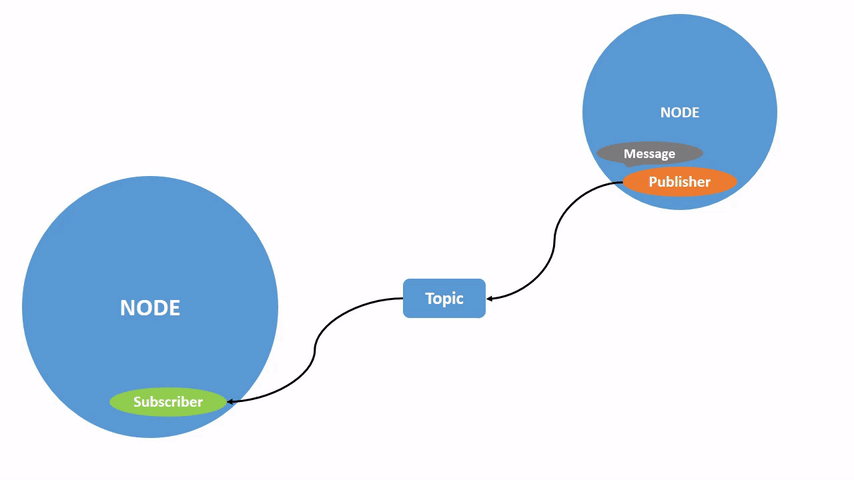
\includegraphics[width=8cm]{img/topicsExplanation.png}
		\caption{Vizualizácia témy v~ROSe~\cite{RosDoc}}
		\label{fig:topics}
	\end{figure}

\newpage
\subsubsection{Služby}
\label{sec:services}

	\textbf {Služby} sú sprostredkované pomocou TCP/IP protokolu. Poskytujú nám rovnaký spôsob komunikácie ako témy, až na~to, že~sa správy
	medzi servisom a~klientom posielajú cez~LAN (\acrlong{LAN}). Tieto správy sa posielajú oboma smermi. Služby sa využívajú pri~komunikácii
	medzi viacerými zariadeniami.

	\begin{figure}[h]
		\centering
		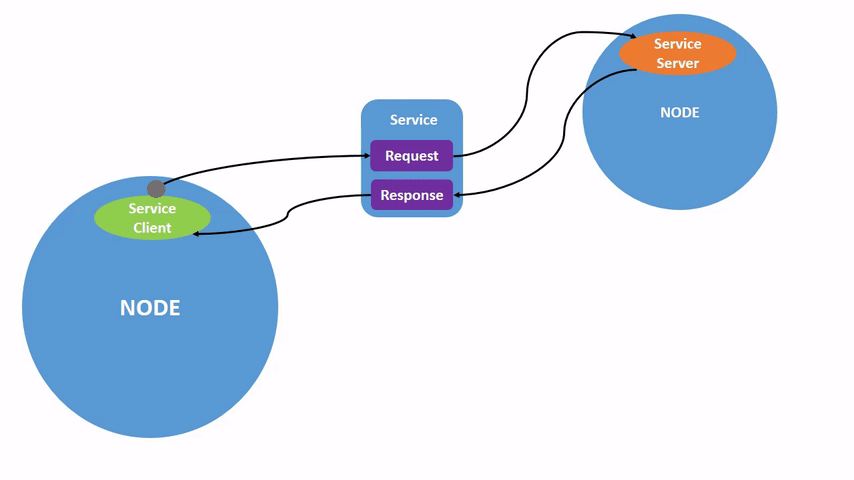
\includegraphics[width=8cm]{img/serviceExplanation.png}
		\caption{Vizualizácia služby v~ROSe~\cite{RosDoc}}
		\label{fig:service}
	\end{figure}

\subsubsection{Akcie}
\label{sec:actions}
	\label{s_action}
	\textbf {Akcie} sú taktiež sprostredkované TCP/IP protokolom. Sú najzložitejším spôsobom komunikácie. Tento spôsob bol pridaný do~ROS1
	až neskôr. V~druhej verzii ROSu je tento typ komunikácie medzi troma základnými formami komunikácie uzlov. Sú založené na~službách
	a~prebiehajú asynchrónne~\cite{ROS2book}. Máju 3 stavy viď Obr.~\ref{fig:action}. Najprv pošle klient serveru, akú akciu má vykonať,
	server mu potvrdí, že~túto požiadavku dostal. Server začne následne vykonávať danú akciu a~posielať klientovi priebežné správy o~priebehu
	vykonávania žiadanej úlohy. Keď server skončí, pošle klientovi výsledok akcie a~klient mu obratom potvrdí obdržanie výsledku.

	\begin{figure}[h]
		\centering
		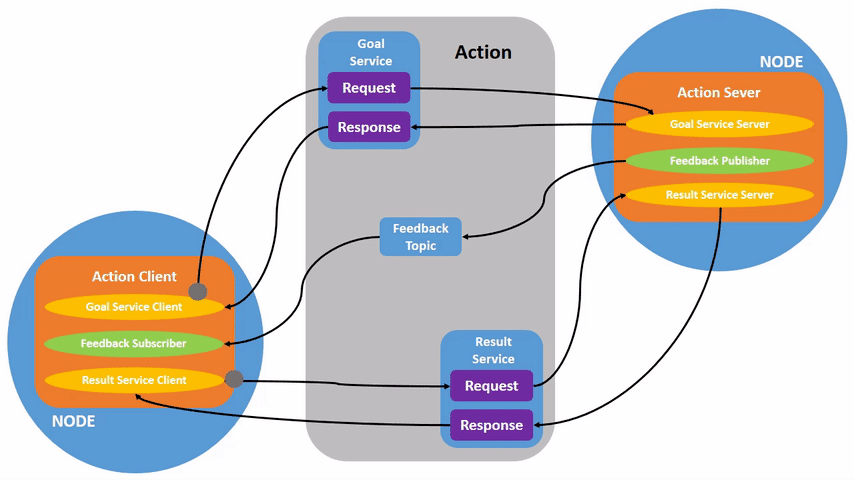
\includegraphics[width=8cm]{img/actionExplanation.png}
		\caption{Vizualizácia akcie v~ROSe~\cite{RosDoc}}
		\label{fig:action}
	\end{figure}

\subsection{Parametre}
\label{sec:parametre}

\textbf{Parametre} sú spôsob, ako môže komunikovať užívateľ so základnými nastaveniami uzlov bez~potreby zmenenia kódu a~jeho
následnej kompilácie, čo pri~väčších projektoch môže zabrať aj trištvrte hodiny. Konfigurácie sa definujú v~\textit{yaml} konfiguračnom
súbore. V~ňom si môžeme zadefinovať mená jednotlivých parametrov a~ich základné hodnoty. Tie si programátor vie v~programe
vytiahnuť pomocou API, \acrlong{API}, (Aplikačné Programovacie Rozhranie) v~ROSe.

\begin{figure}[!htbp]
	\centering
	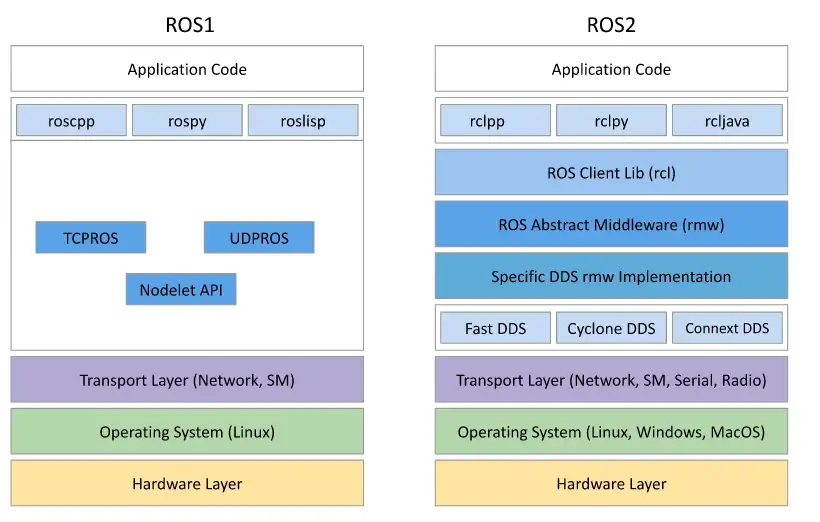
\includegraphics[width=15cm]{img/strukturaRos1Ros2.png}
	\caption{Porovnanie štruktúr ROS1 a~ROS2~\cite{comparison}}
	\label{fig:struktury}
\end{figure}

\subsection{ROS1}

ROS bol prvýkrát vydaný v~roku 2007. Ide o~softvér, ktorý sa začal vyvíjať so zámerom zjednodušiť programovanie a~ovládanie robotov.
Od doby, kedy vznikol prešiel mnohými verziami a~úpravami. Jeho neoddeliteľnou súčasťou sú štrukturovanie programu do~uzlov (nodov),
komunikácia medzi uzlami, podpora viacerých programovacích jazykov ako sú C, C++ alebo Python a~vytváranie balíčkov dostupných širokej
verejnosti.

Štrukturalizovanie základov ROS1 je spravené monoliticky čo najstabilnejším spôsobom. Na~počiatku musí byť spustený hlavný program (roscore),
ktorý zabezpečuje vytváranie jednotlivých uzlov. Komunikácia medzi uzlami je zabezpečená prostredníctvom prepojenia uzlov cez~LAN/WLAN
alebo IPC komunikáciu. Ak sú uzly spustené na~iných zariadeniach, tak~sa využíva len komunikácia cez~sieť. Roscore ďalej poskytuje parametre
jednotlivým uzlom z~parametrového servera. Jeho najdôležitejšou úlohou je zabezpečenie komunikácie uzlov v~programe.

Aj napriek mnohým výhodám má ROS1 aj nedostatky, ktoré sa ťahajú už od~jeho počiatkov. Sú to~napríklad:

\begin{itemize}
	\item Nepostačujúca distribuovanosť systému. Všetky uzly sa spoliehajú na~funkčnosť roscore-u,
	\item ROS1 je písaný v~starom štandarde, to~vnáša do~programu technologický dlh a~bezpečnostné riziká,
	\item Kvalita komunikácie sa nedá ovplyvniť,
	\item Preddefinované vláknové moduly~\cite{ROS2design},
	\item Možnosť užívateľa predefinovať základne prvky ROS-u.
\end{itemize}

Kvôli takýmto problémom a~nedostatkom sa začala vyvíjať nová verzia ROSu, ROS2. Tá mala vyriešiť tieto problémy a~zlepšiť funkcionalitu
prvej verzie. V~roku 2025 sa skončí podpora poslednej distribúcie ROS1 menom \textit{Noetic}. Preto~je odporúčané začínať nové projekty
v~ROS2.

\subsection{ROS2}

Ako už bolo spomenuté zámerom vývoja ROS2 bolo zlepšenie funkcionality a~bezpečnosti systému. Jeden z~dôsledkov tohto vývoja je, že~ROS2
nie je spätne kompatibilný. Podstata toho, ako sú zoskupované uzly a~ako spolu komunikujú je diametrálne odlišná od~ROS1. Z~tohto dôvodu
bol vyvinutý takzvaný rosbridge, ktorý zabezpečuje kompatibilitu medzi verziami. Nie je to~ale trvalé riešenie. Odporúčané je nástroj
využívať a~počas toho prepisovať kód z~verzie 1 do~verzie 2. Komunikácia prebieha v~ROS2 rovnakým spôsobom ako v~ROS1. Pomocou tém
\ref{sec:topic}, služieb \ref{sec:services} a~akcií \ref{sec:actions}.

Táto podobnosť končí na~najvyššej vrstve. Ako sme videli na~Obr.~\ref{fig:struktury}. Štruktúra ROS2 je rozdelená do~viacerých vrstiev.
Najdôležitejšie je pre~nás vedieť, že~komunikácia je spracovávaná modelom DDS (Služba distribúcie údajov) z~anglického (\acrlong{DDS}). Tento
model zlepšuje výkon, stabilitu a~bezpečnosť modelu oproti ROS1. Je založený na~TCP/IP a~UDP/IP protokole. Z~obrázku Obr.~\ref{fig:struktury}
vyčítame aj lepšie rozloženie modulov. To~zabezpečuje jednoduchšie prispôsobovanie systému pre~nové funkcionality. Podpora operačných systémov
sa v~ROS2 rozšírila aj o~Windows, Mac OS či~RTOS (Operačné systémy reálneho času) z~anglického \acrlong{RTOS}. Operačné systémy nie sú jediné
rozšírenie ohľadom kompatibility. S~ROS2 je možné programovať už aj v~Jave či~Matlabe. Tvorcovia mysleli aj na~programátorov a~pridali rozšírené
možnosti testovania, debugovania či~nasadzovania programu do~reálneho využitia.

Testovanie prebieha pomocou použivanie Google testov. Debugovania je možné uskutočniť pomocou debuggera gnu-gdb. Pri~spustení programu
cez~spúšťací súbor (launch file) je potrebné pridať príkaz na~spustenie spomenutého debugovacieho programu.

ROS2 má necentralizovanú štruktúru, a~preto pri~spúšťaní programov už nie je potrebné mať spustený roscore. Ak teda spadne jeden uzol všetky
ostatné uzly budú fungovať naďalej. V~ROS1 sme vedeli ovplyvniť počet uchovaných správ komunikácie pokým nepretiekol zásobník, ktorý ich uchovával
na~neskoršie použitie. V~ROS2 vieme implementovať túto schopnosť použitím takzvanej \textit{QoS} triedy (kvalita komunikácie), z~anglického \acrlong{QoS}.
Pomocou tejto triedy vieme aj zmeniť kvalitu komunikácie. Vieme si zadefinovať, či~by sme radšej stratili niektoré správy, ale dostali by~sme
všetky rýchlo. Alebo aby sa zabezpečilo, že~dostaneme všetky správy, ktoré boli vyslané, aj keby to~trvalo dlhšie. Dokonca si vieme zadefinovať
maximálny čas, ktorý budeme čakať na~ďalšiu správu.

Ak by bol užívateľ veľmi schopný programátor a~potreboval by si zmeniť triedy, ktoré definujú základnú funkcionalitu ROS-u, tak~aj toto je možné.
Jednou z~takýchto funkcionalít je, že~užívateľ si vie predefinovať triedu, ktorá bude alokovať miesto na~(IPC) komunikáciu (medziprocesovú komunikáciu).
K~tomuto bodu je dodať, že~tento prípad je špecifický a~väčšina programátorov sa s takouto možnosťou do~kontaktu nedostane.

Pri~všetkých týchto zlepšeniach nemôžeme zabudnúť spomenúť aj nasledovný nedostatok. Keďže ROS2 je mladší ako ROS1 nájdeme k~nemu menej dokumentácie.
Pridaním veľkého počtu funkcionalít začal vznikať problém pre~začiatočníkov s~porozumením niektorých kódov. Avšak tento problém je nedostatkom,
ktorý časom zanikne. V~čase písania tejto práce pribudli na~stránke dokumentácie minimálne 2 strany popisujúce pokročilejšie Funkcionality druhej
verzie ROSu.

\subsection{Rozdiely}

Čo je určite dobrou správou pre~všetkých programátorov, ktorí robili v~prvej verzii a~sú zvyknutí na~jej štandardy a~funkcionalitu. Tak títo
sa nemajú čoho obávať. Prechod z~ROS1 na~ROS2 je dosť priamočiary. Čo sa zmenilo je spôsob písania kódu, ale koncepty ostali všetky rovnaké.
V~tejto sekcii nebudeme písať konkrétne kódy, budeme len opisovať čo je podobné a~čo zasa rozdielne medzi verziami spomínaného systému. Keďže
celý projekt bol písaný v~programovacom jazyku C++ tak~sa aj tieto zmeny budu týkať hlavne jazyka C++.

\subsubsection{Štandard jazyka}

	Pokým ROS1 bola písaná v~štandarde C++03 tak~ROS2 je už písaná v~novom štandarde. A~to hlavne C++11, ale používa aj nejaké časti z~C++14
	a~C++17. To~zahŕňa inicializovanie templatov a~ich používanie. Tým, že~ROS2 je stále nová a~stále vyvíjajúca sa platforma, tak~môžeme očakávať aj časti
	kódu, ktoré budú podporovať najnovší C++ štandard a~to štandard z~rokov 2020 a~2023.

	Definície a~deklarácie templatov sú na~knihu samú o~sebe, preto do~detailov nebudeme zachádzať. Stačí nám vedieť, ako ich inicializovať.
	V~prvej verzii sme definovali všeobecného publishera (publikovateľa) a~definovali sme mu len cez~akú tému má posielať správy. V~druhej verzii
	naväzujeme publishera na~špecifický tip správy akú posielame. Nemôže sa teda stať, že~takýto program by sme skompilovali a~následne, keď
	ho spustíme, tak~by spadol z~dôvodu, že~čítame iný typ správy ako posielame.

\subsubsection{Inicializácia nody (uzla)}

	Tak isto ako v~prvej verzii aj v~druhej verzii musíme definovať uzol (node). Rozdiel je v~tom, že~prvá verzia obsahovala NodeHandle (Ovládač uzla)
	a~druhá verzia obsahuje priamo Node (Uzol). V~druhej verzii je zaužívaným štandardom túto nodu predediť a~použiť polymorfizmus pri~objekte,
	ktorý bude existovať počas celej doby vykonávania programu. Pri~prvej verzii tomu tak~nebolo. Tam sme museli vytvoriť už spomenutý NodeHandle.
	Ten sa nemusel využiť ako base trieda a~nemusel ani~existovať počas celého behu programu.

\subsubsection{Komunikácia}

	DDS (Služba distribúcie údajov) je protokol strednej vrstvy (middleware) implementovaný nad UDP~\cite{ROS2book}. Na implementáciu tohto protokolu
	je použitý protokol z~IoT (internet veci) (\acrlong{IoT}) sféry. Je to protokol MQTT. DDS je používaný v~ROS2 na~komunikáciu medzi uzlami. Je
	to~systém správ publikovania (publish) / odoberania (subscribe), ktorý umožňuje uzlom komunikovať medzi sebou bez toho, aby poznali identitu
	ostatných uzlov. Druh komunikácie je v~ROS2 rozšírený ešte o~akcie viď~\ref{s_action}.

\subsection{Parametre}

	ROS1 používa parametrový server, ktorý sa nachádza v~roscore-e. Každý uzol si mohol vytiahnuť parametre, ktoré boli zapísané v~konfiguračnom
	súbore. ROS2 žiadny roscore nemá, preto sa parametre musia distribuovať iným spôsobom. Parametre v~druhej verzii ROSu patria jednotlivým uzlom.
	To~znamená, že~jednotlivé parametre sa dajú vytiahnuť len daným uzlom. Tieto parametre taktiež existujú len počas existencie daného uzlu. Parametre
	sú ďalej distribuované pomocou už spomínaného DDS protokolu. V~prípade, že~sa tieto parametre nepodari vytiahnuť z~konfiguračného súboru. Či už z~dôvodu,
	že daný súbor neexistuje, alebo iného dôvodu, tak~sa aplikujú základné hodnoty, ktoré si zvolil užívateľ pri~používaní funkcie na~ich zisťovanie.

\subsubsection{Nodelet alebo komponent}

	ROS1 ponúka možnosť definície uzlov ako uzlík (\texttt{nodelet}). Je to~definovanie uzlu ako zdielanej knižnice (shared library). Je
	to~spôsob ako uľahčiť prácu CPU. Keď sa definuje uzol ako uzlík, tak~jeden proces môže spracovávať programy z~viacerých takýchto uzlíkov.
	Táto funkcionalita sa nachádza aj v~ROS2. Volá sa komponent (\texttt{component}). Vylepšením oproti nodelet-om je zjednotenie aplikačnej
	implementácie (API). Pokým nodelet-y mali vlastný spôsob implementácie v~ROS1 tak~v~ROS2 je implementácia uzla a~komponentu rovnaká.
	Pri~komponente sa musí len naviac definovať, že~daný komponent existuje pomocou makra. Použitie komponentov zjednodušuje prácu CPU
	a~používa sa hlavne v~zariadeniach, ktoré majú obmedzený výkon výpočtovej techniky. Sú to napríklad mikroprocesory, ktoré ovládajú roboty.

\subsubsection{Kompilácia}

	Zmenou verzii sa zmenil aj spôsob kompilácie programu. ROS1 bol kompilovaný pomocou \texttt{catkin} build systému. Catkin je založený
	na~programe \texttt{cmake}. Jeho nastavenie dependencií je konfigurované pomocou súboru \texttt{package.xml}. ROS2 prešiel na~viac
	nastaviteľný systém \texttt{Colcon}. Tento systém je na~rozdiel od~catkin-u založený na~Python-e a~jeho dependencie sa nastavujú pomocou
	\texttt{setup.py} súboru. V~prípade colcon-u si môžeme definovať spôsob kompilácie to~znamená, že~môžeme nastaviť, ako sa budú spracovávať
	dependencie. Ponúkané možnosti sú \texttt{catkin\_make}, \texttt{catkin\_make\_isolated}, \texttt{catkin\_tools} a~\texttt{ament\_cmake}.
	Jednou s~najviac používaných možností je \texttt{ament\_cmake}. Je založený na~programe \texttt{cmake} a~spolupracuje so systémom \texttt{colcon}.
	Z~tohto dôvodu mu vieme definovať dependencie pomocou xml súboru ako tomu bolo v~ROS1 pričom možnosť definície pomocou Python skriptu ostáva.
	Je to~jeden zo spôsobov, ako zmenšiť rozdiel medzi ROS1 a~ROS2.

\subsubsection{Vlákna}

	ROS1 dovoľuje programátorom vybrať si medzi jedno vláknovým a~viac vláknovým vykonávaním programu. Tvorcovia ROS2 si dali zaležať na~modularite
	aj tejto oblasti kódu. V~druhej verzii ROS-u si vieme zadefinovať typ vykonávania programu separátne pre každý uzol a~vieme si tento typ
	zadefinovať aj sami~\cite{ROS2design}.

\section{Robot a~jeho ovládanie}

Robot, s~ktorým sme pracovali bol výsledkom tímového projektu viacerých študentov \newline z~roku 2019. Pri~vysvetľovaní a~opisovaní robota sa budeme
odvolávať na~dokumenty, stránky a~kód, ktorý napísali. Všetky tieto údaje si sprístupnené na~mobilnom robote v~záložke
\newline \texttt{\$(HOME)/Desktop/Blackmetal}~\cite{timovyProjekt}.

Robot je v~tvare kvádra. Jeho šírka je 60cm a~je vyzdvihnutý nad zem o~1.5cm. Nachádza sa na~kolesách o~polomere 8cm. Jeho kostra, až na~oceľové pláty,
ktoré držia robot, je spravená z~hliníku. Konkrétne z~hliníkových tyčí, ktoré sú pospájané plexisklovými plátmi. Jeho podobizeň vidíme na~nasledujúcom
obrázku.

\begin{figure}[!htbp]
	\begin{center}
		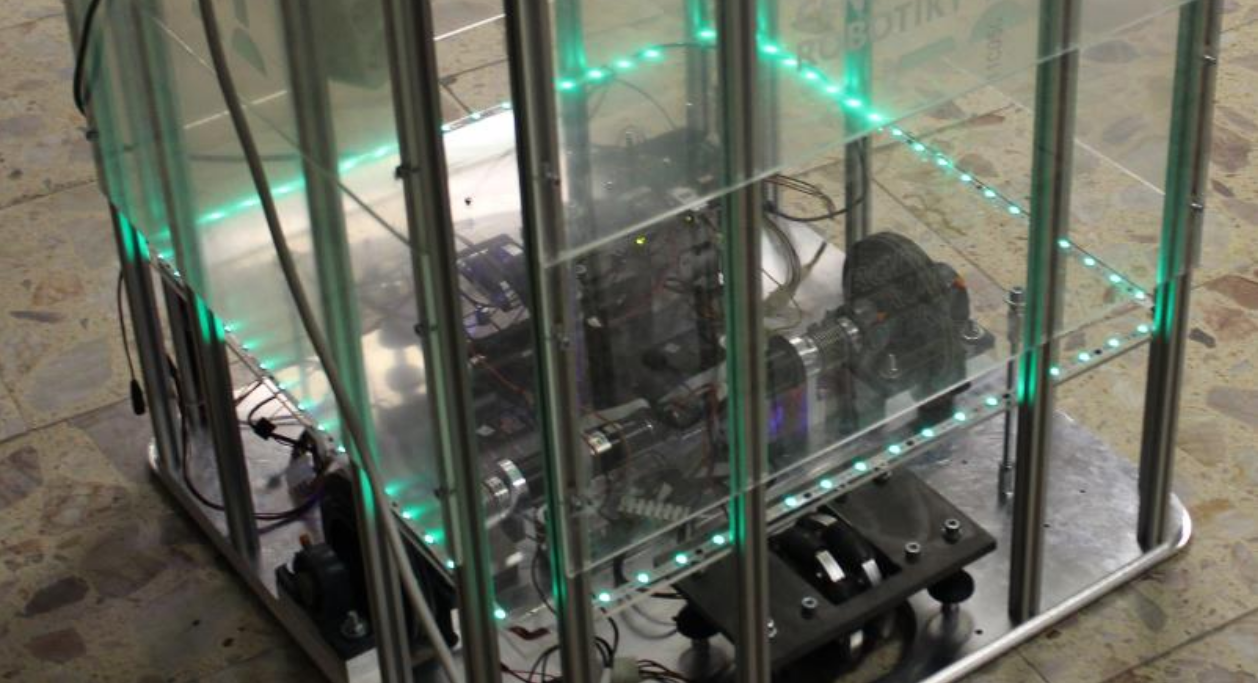
\includegraphics[width=0.95\textwidth]{img/robot.png}
	\end{center}
	\caption{Zobrazenie spodnej časti mobilného robota~\cite{timovyProjekt}}
	\label{fig:robot}
\end{figure}

\noindent Na~obrázku ďalej vidíme olemovanie robota pásom s~LED-kami. Tie svietia nasledovným spôsobom. Keď sa robot nehýbe všetky LED-ky svietia
na zeleno. Keď sa robot pohne do~nejakej strany, LED-ky znázornia jeho pohyb tým, že~svietia na~strane, do~ktorej sa robot hýbe. Keď nastane
situácia, kedy počítač ovládajúci motory prestane komunikovať s~Arduinom, ktoré sa stará o~detekciu stavov robota tak~LED-ky začnú blikať
červeno-modrými farbami.

Ako bolo spomenuté LED-ky znázorňujú pohyb robota. Ten sa pohybuje za pomoci diferenciálneho podvozku s~dvoma podpornými všesmerovými kolesami.
Motory robota sú pripojené na~meniče. Tie sú ovládané priamo príkazmi z~počítača.

\subsection{Hardware}

Hardware robota sa skladá z:
\begin{itemize}
	\item kontrolnej dosky Arduino Uno,

	\item Počítača ADVANTECH MIO-5272~\cite{robotPc} \newline
		Počítač obsahuje operačný systém Ubuntu 16.04.

	\item Extension board MIOe-210~\cite{extensionModule}

	\item Meniče MAXON EPOS 24/5 (s číslom 275512)~\cite{menic} \newline
	 	Sú napájané jednosmerným napätím 11 - 24 V~a~5 A.

	\item Enkódery MAXON Encoder MR Type L (s číslom 225787)~\cite{encoder} \newline
		Rozlíšenie enkóderov je 1024 impulzov s~troma kanálmi.

	\item Motory MAXON RE 40 (s číslom 148867)~\cite{motor} \newline
		Motory s~výkonom 150W. Maximálna rýchlosť je 12 000 rpm a~efektivita 91\%.

	\item Prevodovka MAXON Planetary Gearhead GP 42 C (s číslom 202120)~\cite{prevodovka} \newline
		Redukcia prevodovky je 43:1. Jej účinnosť je 72\%.
\end{itemize}

\noindent Ovládanie robota je zabezpečené externými počítačmi
\begin{itemize}
	\item Control PC (Kontrolný počítač) -- Počítač posielajúci príkazy na~robot cez~TCP/IP protokol.
	\item Logging PC (Logovací počítač) -- Počítač prijímajúci stav robota cez~TCP/IP protokol.
\end{itemize}

\begin{figure}[!htbp]
	\begin{center}
		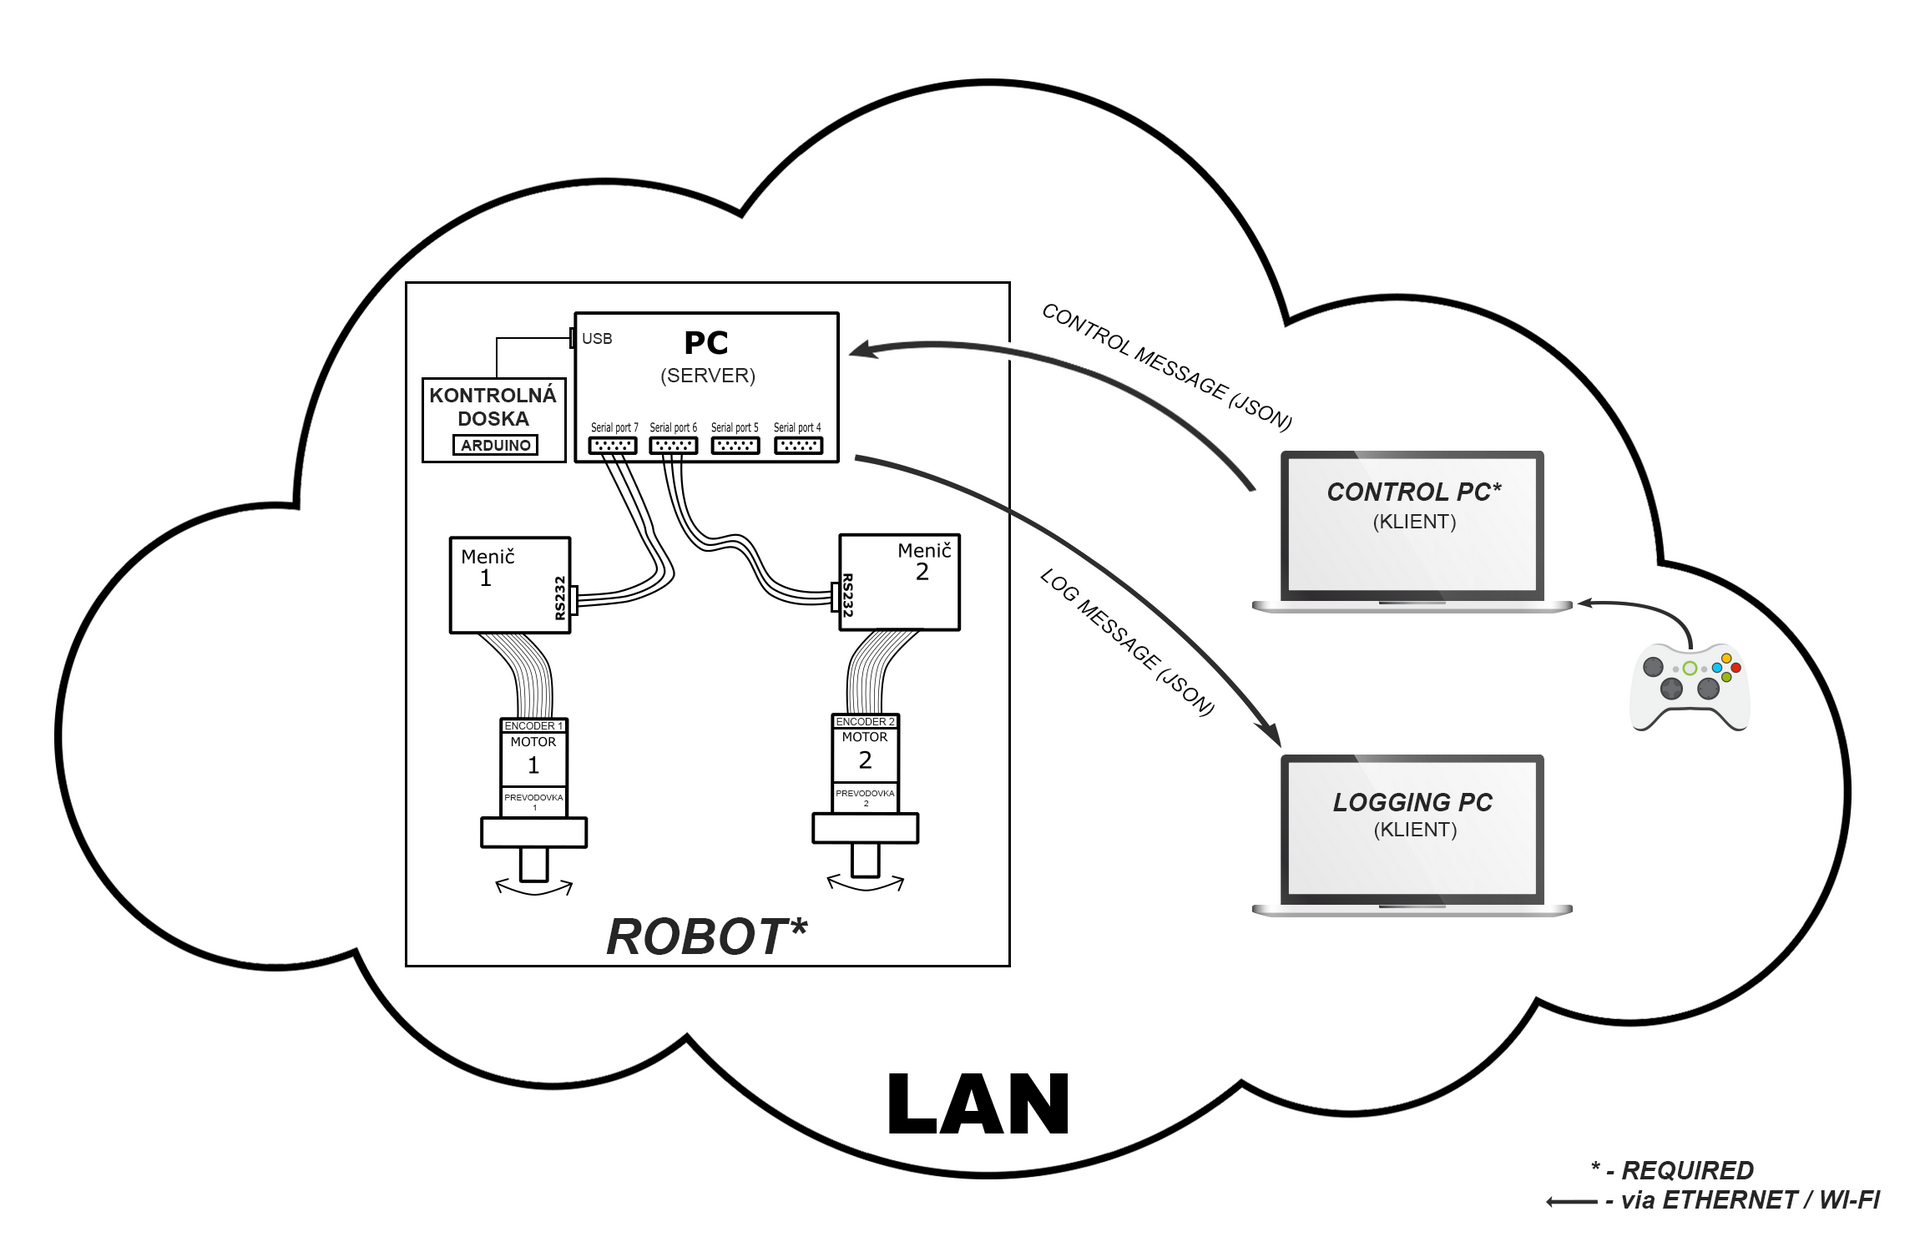
\includegraphics[width=9cm]{img/schemaRobota.png}
	\end{center}
	\caption{Schéma zapojenia jednotlivých častí na~robote}
	\label{fig:schemaRobota}
\end{figure}

\noindent Tieto počítače sú len reprezentácia servera. V~realite to môže byť jeden a~ten istý počítač.

\noindent Na obrázku Obr.~\ref{fig:schemaRobota} vidíme zapojenie jednotlivých častí robota. Čo sme nespomenuli a~je na~obrázku je XBox ovládač
je to~kvôli tomu, že~tímový projekt bol zameraný na~ovládanie robota pomocou tohto ovládača. My ho ale použivať nebudeme.

\subsection{Komunikácia s~robotom}

S robotom sa vieme spojiť pomocou dvoch portov. Jeden port je otvorený na~prijímanie požiadavok (requestov) a~ten druhý je na~monitorovanie
stavu robota. Port \textit{664} je otvorený pre~tisíc užívateľov, ktorí môžu len sledovať stav robota. Druhý port je na~prijímanie requestov
\textit{665} a~je otvorený len pre~jedného užívateľa.

\subsubsection{Logovanie}
\label{sec:logovanie}

	Spomínaný port \textit{664} je otvorený jednému užívateľovi. Keď sa užívateľ pripojí začne dostávať nepretržite správy typu
	\textit{JSON}~(\acrlong{JSON}), ktoré hlásia stav robota. Správy, ktoré dostávame sú nasledujúceho formátu

	\begin{lstlisting}
			{"state":1,"direction":1}
	\end{lstlisting}

	Hodnoty sa pri~stave (state) a~ani pri~smere (direction) nemenia. Sú to~stále jednotky. Pokým robota nezastavíme buď príkazom, stlačením
	tlačidla vypnutia alebo zablokovaním jedného z~kolies, tak~sa tieto správy budú posielať. Môžeme potom začať polemizovať o~tom či~by nebolo
	lepšie už tieto správy využiť na~to~čo reálne spomenutý \textit{JSON} reťazec ukazuje. A~to udávať smer a~stav robota. Momentálne tieto správy
	slučia len na~to, aby sme vedeli, že~tento robot je aktívny a~vie primať a~spracúvať informácie.

\subsubsection{Ovládanie}
\label{sec:ovladanie}

	Port \textit{665} je sprístupnený na~prijímanie a~odosielanie požiadavok a~ich odpovedí. Príkazy sa na~počítač posielajú cez~sieť z~externého
	počítača vo~formáte \textbf{JSON}. Študenti, ktorí navrhovali systém posielania požiadavok (request) a~odpovedí (response) robili tieto správy
	ručne. Preto~nastávajú situácie, kedy robot pošle správu, ktorá nespadá do~štandardu písania JSON textu. Z~tohto dôvodu sme nemohli použiť už
	existujúci kód (parser), ktorý by nám zjednodušil prehľadávanie týchto správ. Podla dokumentácie sa robot mal ovládať správami typu~\cite{BMdoc}

	\label{jsonSpeedRequestBad}
	\begin{lstlisting}
			{"UserID":1,"Command":3,"RightWheelSpeed":50,"LeftWheelSpeed":50}
	\end{lstlisting}

	\newpage

	\noindent Význam jednotlivých parametrov:
	\begin{itemize}
		\item \textbf{UserID} -- Znázorňuje ID užívateľa, ktorý je pripojený na~robot. Predvolená hodnota je 1.
		\item \textbf{Command} --  Číselná hodnota znázorňujúca príkaz, ktorý ma robot vykonať
			\begin{enumerate}
				\setcounter{enumi}{-1}
				\item \label{c0} Prázdny príkaz slúžiaci na~overenie spojenia
				\item \label{c1} Núdzové zastavenie
				\item \label{c2} Normálne zastavenie
				\item \label{c3} Príkaz nastavujúc rýchlosti kolies mobilného robota
				\item \label{c4} Prázdny príkaz
				\item \label{c5} Prázdny príkaz
				\item \label{c6} Príkaz pýtajúci si aktuálnu rýchlosti pravého a~ľavého kolesa. Tento príkaz nebol sprave navrhnutý v~kóde
					robota. Vracal nám žiadaná hodnotu namiesto aktuálnej. Museli sme ho prepísať.
				\item \label{c7} Pripravenie motorov robota
				\item \label{c8} Príkaz pýtajúci si aktuálnu pozíciu pravého a~ľavého kolesa.
			\end{enumerate}
		\item \textbf{RightWheelSpeed} -- Nastavenie rýchlosti pre~pravé koleso
		\item \textbf{LeftWheelSpeed} -- Nastavenie rýchlosti pre~ľavé koleso
	\end{itemize}

	\noindent Z~tohto kusu kódu je jasné, že~sa majú posielať celé čísla a~na základe tohto vstupu sa bude robot hýbať. Čo sme zistili až
	po skompilovaní a~spustení tímového projektu je, že~sa majú posielať desatinné čísla z~intervalu 0 až 1. Toto nebolo písané
	v~dokumentácii, ktorá nám bola dodaná na~začiatku programu. Môžeme preto príklad prepísať na~reťazec, ktorý by fungoval

	\label{jsonSpeedRequestGood}
	\begin{lstlisting}
			{"UserID":1,"Command":3,"RightWheelSpeed":0.50,"LeftWheelSpeed":0.50}
	\end{lstlisting}

\subsection{Vysvetlenie kľúčov reťazca}

\noindent \textbf{UserID} \newline
\indent Táto možnosť je v~momentálnom stave robota nevyužitá. Počet zariadení, ktoré sa môžu pripojiť na~port, cez~ktorý sa dá robot ovládať
je 1. Je to~ale dobrá možnosť na~rozšírenie kódu. Keď sa budú môcť pripojiť viacerí užívatelia, tak~sa bude musieť vyriešiť, koho príkaz
bude mať akú prioritu. \newline

\noindent \textbf{Command:~\ref{c4}} \newline
\indent Tento príkaz je prázdny. My sme ho ale neskôr prepísali na~príkaz, cez~ktorý sa dá nastaviť žiadaná pozícia kolies robota (natočenie).
Táto funkcionalita nie je v~takom stave ako sme si priali. Je to spôsobené hlavne nedostačujúcov dokumentáciou enkóderov na~robote. Síce sme našli
v~dokumentácii funkciu, ktorá by mala túto možnosť povoľovať. Čo sa ale stane pri~poslaní príkazu je to, že~kolesá sa začnú točiť rýchlosťou
0,5 metra za sekundu.\newline

\noindent \textbf{Command:~\ref{c8}} \newline
\indent Príkaz na~zisťovanie polohy kolies nebol originálne naprogramovaný na~robote. Pridali sme ho za cieľom presného dostavia sa robota
na~preddefinované miesto. Táto funkcionalita nefunguje správne rovnako ako v~predchádzajúcom príklade, keď si vypýtame polohu kolies od robota,
dáta ktoré obdržme sú, že~jedno koleso je priamo nastavené na~hodnotu, ktorú sme si vyžiadali a~to druhé koleso vráti náhodnú hodnotu.
Počas toho sa ale kolesá robota stále točia.\newline

\noindent \textbf{RightWheelSpeed/LeftWheelSpeed} \newline
\indent Nastavovanie rýchlosti pravého a~ľavého kolesa nie sú povinné parametre. Musíme ich zadávať len v~prípade posielania rýchlostí
cez~príkaz s~číslom \ref{c3} alebo \ref{c4}.

\subsection{Oprava chýb na~robote}

\subsubsection{Nesprávna funkcia}

Ako bolo spomenuté vyššie, pri~poslaní príkazu s~číslom~\ref{c6} nám robot vráti aktuálne rýchlosti kolies. Počas skúšania tejto funkcionality
sme narazili na~problém. Keď sme sa robota spýtali na~jeho rýchlosti. Dostali sme reťazec, ktorý obsahoval náhodne veľké čísla. Tieto čísla sa
menili, keď sme zadávali nejaké hodnoty pre~rýchlosti kolies aby~sa robot hýbal. Ich magnitúda ostávala rovnaká. V~nasledujúcom príklade môžeme
vidieť ako tento reťazec vyzeral:

\label{jsonWannabeSpeed}
\begin{lstlisting}
		{"LeftWheelSpeed"=236223201280 "RightWheelSpeed"=4294967296}
\end{lstlisting}

Tu vidíme príklad obdržanej správy. Ako si môžeme všimnúť. Pri~tomto type správ nie je dodržaná správna forma reťazca typu JSON. Namiesto `:'
máme `=' a~medzi argumentmi sa nenachádza čiarka. Hneď ako prvú vec sme chceli tento štandard napraviť. Bohužiaľ na~tomto robote už~bolo
spravených niekoľko projektov a~museli by sme prejsť každý z~nich a~zistiť či~používajú túto spätnú väzbu. Ak~by ju používali museli by sme
tieto kódy upraviť.

\newpage

V~dokumentácii robota bohužiaľ nebolo písané v~akom formáte sa tieto rýchlosti kolies majú nachádzať. Preto jeden z~nápadov ako zistiť presne
v~akom formáte sa posielali tieto čísla bolo vyskúšať pár možností. Boli to

\begin{itemize}
	\item \textit{long} - celé číslo s malým endianom
	\item \textit{long} - celé číslo s veľkým endianom
	\item \textit{float} - desatinné číslo s malým endianom
	\item \textit{float} - desatinné číslo s veľkým endianom
\end{itemize}

Keďže robot má počítač so~63 bytovým procesorom \cite{robotPc}, tak~\textit{long} aj~\textit{float} budú mať 64 bitovú dĺžku. Po~skúsení všetkých
štyroch možností sa~ukázalo, že~ani jedna nebola správna a~problém je niekde inde.

Problém je v~tom, že~keď posielame request na~nastavenie rýchlosti kolies, tak~kód na~robote funguje tak, že~si ich premení na~celé čísla v~rozsahu
0~až~1000. To~je hodnota, na~ktorú nastaví rýchlosti otáčania pravého a~ľavého kolesa respektíve rýchlosť otáčania ich motorov. Na~druhú stranu,
keď si vypýtame od~robota rýchlosti kolies. On zoberie informáciu z~enkóderov a~pošle nám ju~bez spracovania. Aj napriek týmto poznatkom sa nám
nepodarilo získať z~týchto dát žiadané rýchlosti.

Po dôkladnom preštudovaní kódu sme zistili, že~hodnoty ktoré nám posiela robot nie sú ani~vyťahované z~enkóderov správnou funkciou. Preto~sme ju
zmenili a~začali sme dostávať hodnoty, s~ktorými by sa mohlo dať pracovať.

Funkcie z~knižnice zabezpečujúce komunikáciu z~enkóderov motorov pochádzajú z~firmy Maxon~\cite{EPOSdoc}. Táto dokumentácia nebola moc nápomocná.
Opisy jednotlivých funkcií boli len~ich rozložené názvy na~osobitné slová. Aj~napriek tomu sa nám podarilo nájsť funkcie, ktoré sme potrebovali.
Funkcie, ktoré končia koncovkou `Target', alebo toto slovo obsahujú, majú návratné hodnoty reprezentujúce žiadané hodnoty. Funkcie s~koncovkou
`Is' vracajú aktuálne hodnoty. Z~tohto dôvodu sme museli prepísať funkciu na~robote, ktorá sa vykonávala, keď sme chceli získať aktuálne hodnoty
rýchlosti motora poslaním príkazu \ref{c6}. Funkciu, ktorú sme zmenili môžeme vidieť v~nasledujúcej ukážke:

\lstset{language=C++,
	basicstyle=\ttfamily,
	keywordstyle=\color{blue}\ttfamily,
	stringstyle=\color{red}\ttfamily,
	commentstyle=\color{green}\ttfamily,
	morecomment=[l][\color{magenta}]{\#},
	numberstyle=\color{orange}
}

\label{VelocityIs}
\begin{lstlisting}[language=C++]
BOOL VCS_GetTargetVelocity(
	HANDLE KeyHandle,
	WORD NodeId,
	long* pTargetVelocity,
	DWORD* pErrorCode);
\end{lstlisting}

\begin{lstlisting}[language=C++]
BOOL VCS_GetVelocityIs(
	HANDLE KeyHandle,
	WORD NodeId,
	long* pVelocityIs,
	DWORD* pErrorCode);
\end{lstlisting}

\noindent Ako môžeme vidieť v~týchto predpisoch funkcií, bolo treba zmeniť názov funkcie a~ostatné parametre ostali rovnaké.
Nebolo treba meniť implementáciu kódu.

\subsubsection{Zašumený výstup}

Po~prepísaní funkcie na~získavanie rýchlostí robota sme spravili pár meraní, aby sme zistili, aké presné informácie o~rýchlostiach
motorov dostávame. Aby nám robot neodbiehal postavili sme ho na~vyvýšené miesto, tak~aby sa kolesá nedotýkali zeme. V~takomto
postavení sa robot nepohne z~miesta a~my môžeme bez~problémov odmerať prechodové a~prenosové charakteristiky rýchlosti pravého
a~ľavého motora.

\begin{figure}[!htbp]
	\begin{subfigure}{0.5\textwidth}
		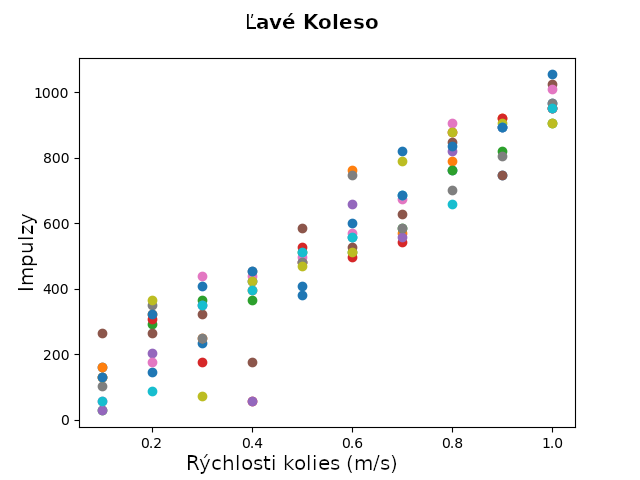
\includegraphics[width=\textwidth]{img/Left_wheel_2.png}
	\end{subfigure}
	\hfill
	\begin{subfigure}{0.5\textwidth}
		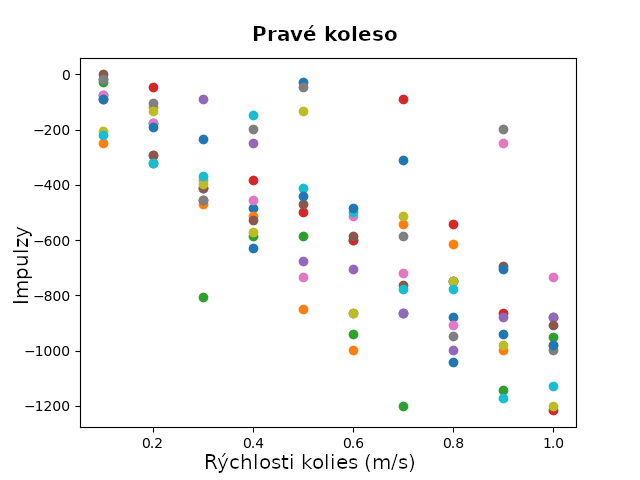
\includegraphics[width=\textwidth]{img/Right_wheel_2.png}
	\end{subfigure}
	\caption{Ustálené hodnoty rýchlosti ľavého a~pravého motora. }
	\label{fig:lavePraveKoleso}
\end{figure}

Po~obdržaní takýchto dát sme kontaktovali jedného z~autorov tímového projektu~\cite{timovyProjekt}, Adriána Kasperkevic. On nám odpísal s~tým,
že~aj oni mali problémy s~enkódermi. Na obrázku Obr.~\ref{fig:prechChar} vidíme zašmený signál rýchlosti poskytovanú enkódermi. Ich problémy
boli naviazané na~staré enkódery, ktoré neskôr vymenili. Na~nových enkodéroch avšak netestovali ich spätnú väzbu.

\begin{figure}[!htbp]
	\begin{center}
		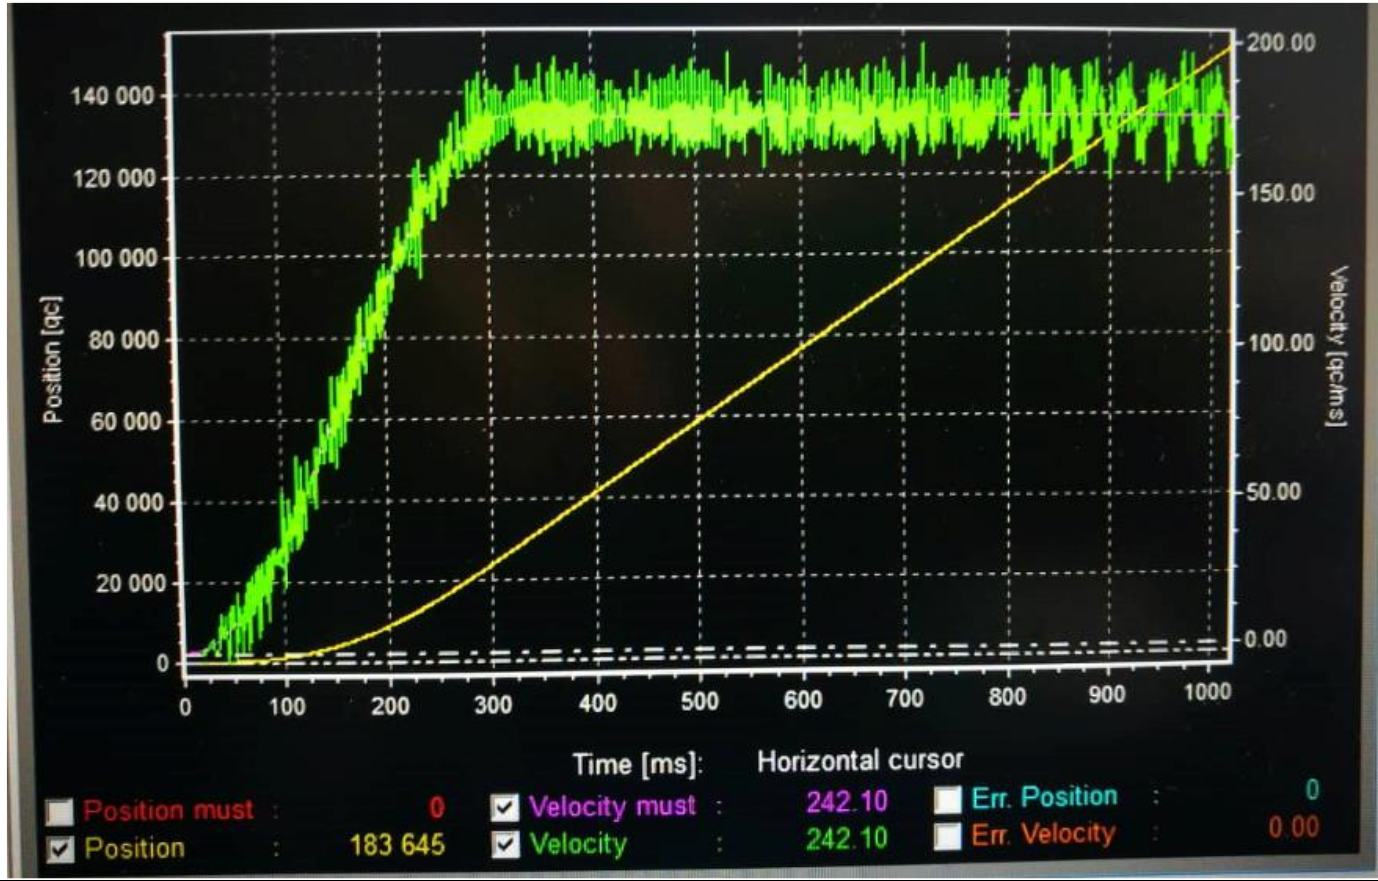
\includegraphics[width=0.95\textwidth]{img/robotSpeedChar.png}
	\end{center}
	\caption{Prechodová charakteristika rýchlosti kolies~\cite{timovyProjekt}. }
	\label{fig:prechChar}
\end{figure}

\section{Implementácia ovládača}
\label{sec:program}

\begin{figure}[!htbp]
	\begin{center}
		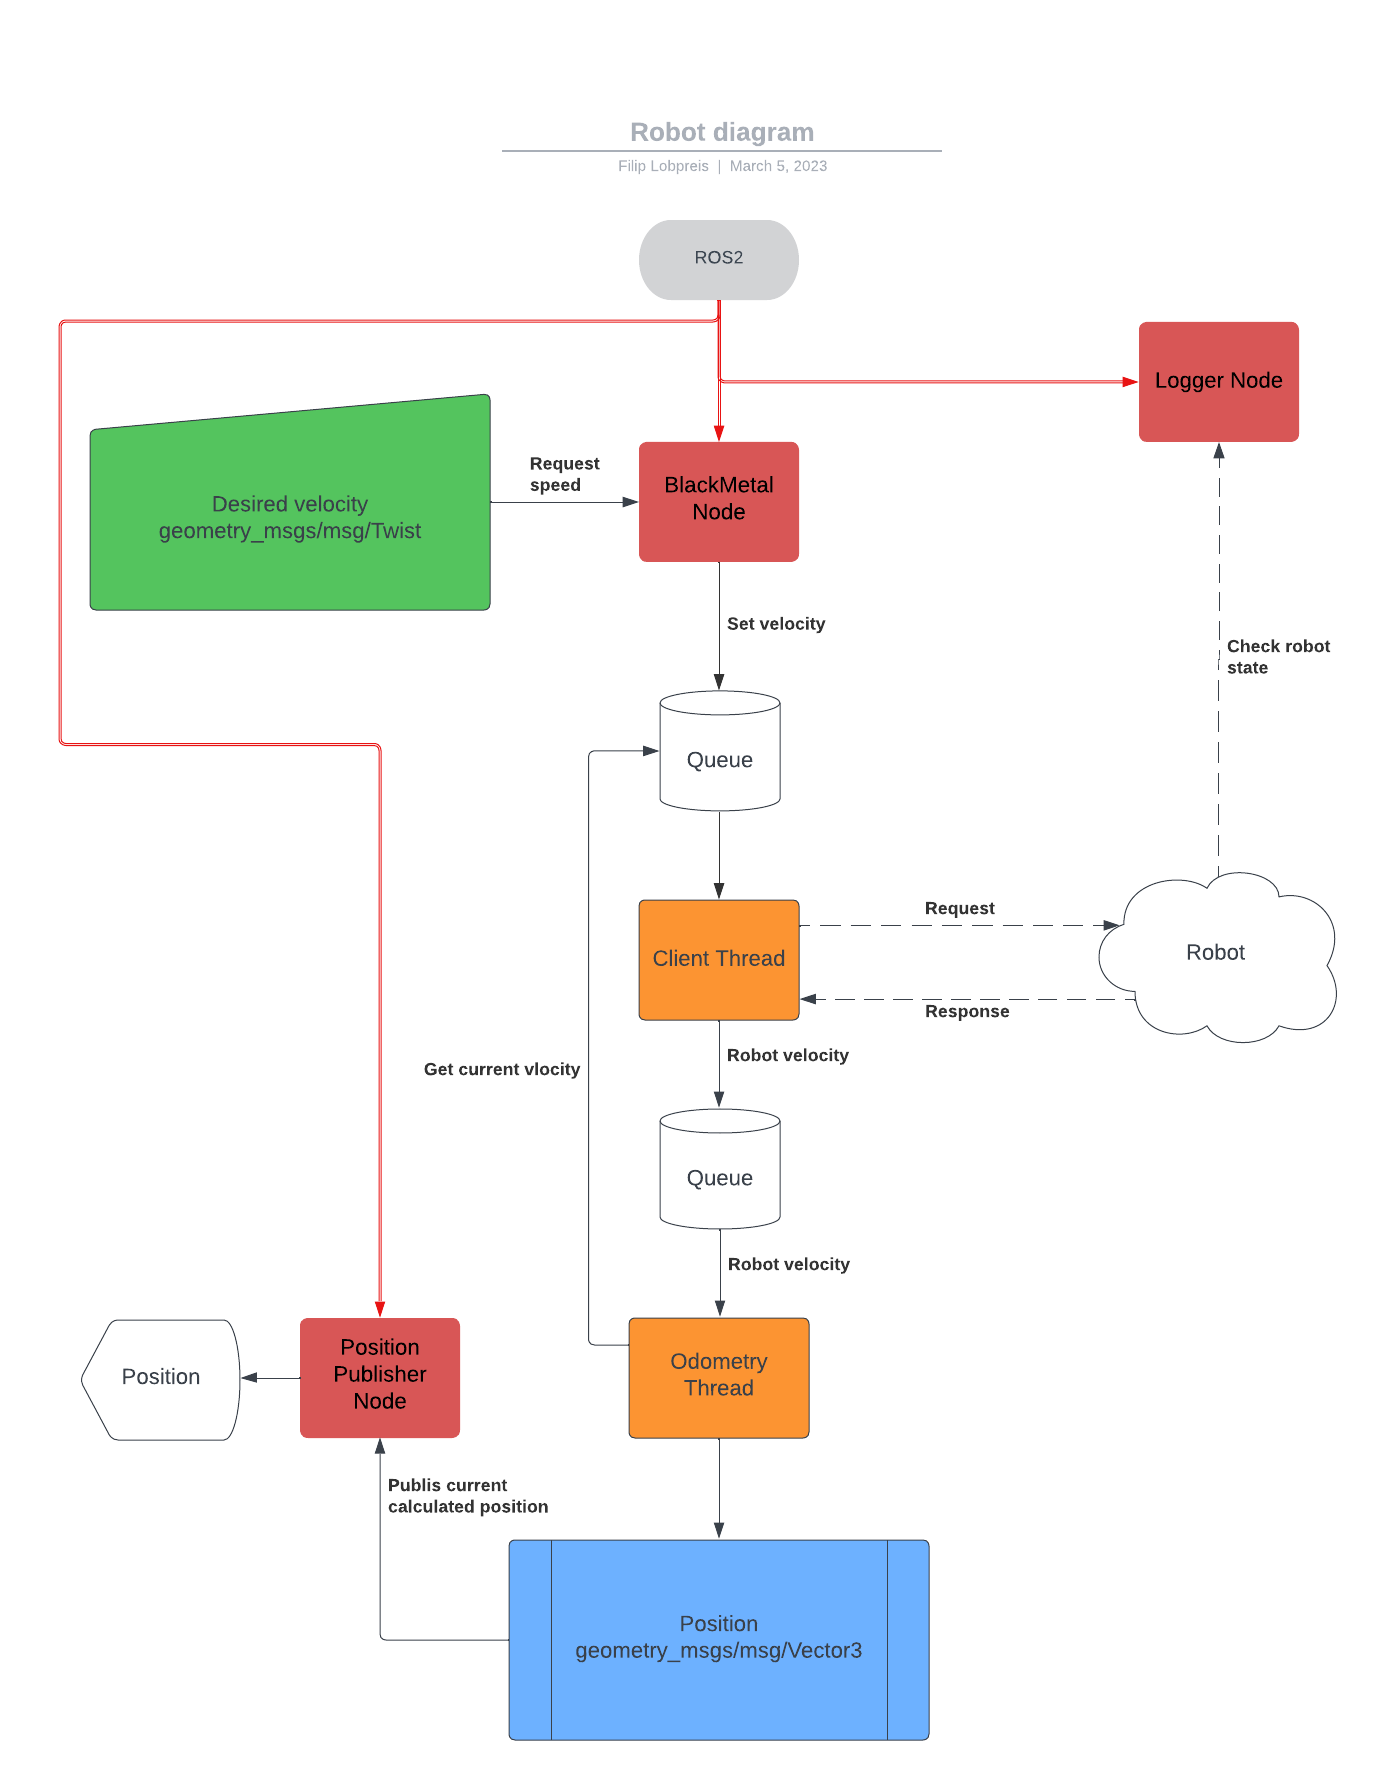
\includegraphics[width=0.9\textwidth]{img/BlackMetal_flowchart.png}
	\end{center}
	\caption{Graf vykonávania programu na~ovládanie robota pomocou ROS2.}
	\label{fig:flowchart}
\end{figure}

\subsection{Úvod do~čítania grafu}
\label{sec:citanie_grafu}

Na~obrázku Obr.~\ref{fig:flowchart} môžeme vidieť viacero objektov rôznych farieb. Objekty zobrazené červenou farbou sú uzly spracovávané
a~vytvárané v~rámci ROS2. Každý tento objekt sa vykonáva v~osobitnom procese. Objekty zobrazené oranžovou farbou sú objekty, ktoré majú svoje
vlastné vlákno. Tieto objekty boli vytvorené uzlom BlackMetal. Dátové štruktúry Queue, zobrazené bielou farbou sú vytvorene  tak~aby
zabezpečovali bezchybnú komunikáciu medzi viacerými vláknami. Objekt so zelenou farbou je vstup do~programu. Je zadávaný užívateľom
a~reprezentuje žiadanú rýchlosť robota. Modry objekt je výstupom programu. Je to téma, na~ktorý sa publikuje aktuálna pozícia robota.
Robot samotný je zobrazený bielou farbou vo~forme malého obláčika. Prerušované čiary na~diagrame znázorňujú sieťovú komunikáciu programu
a~robota. Červené dvojité čiary udávajú, ktoré objekty patria ROS-u. Nakoniec čierne plné čiary reprezentujú tok dát medzi objektami.

\subsection{Uzly}

Na~obrázku Obr.~\ref{fig:flowchart} môžeme vidieť postup vykonávania programu na~ovládanie robota BlackMetal pomocou ROS2.
Na~začiatku programu sa vytvoria 3 uzly. Prvý uzol \textbf{Position Publisher Node} je uzol, na~ktorý sa publikuje vypočítaná pozícia robota.
Počíta sa na~základe obdržaných dát z~enkóderov robota. Uzol \textbf{Logger Node} slúži na~zaznamenávanie stavu robota \ref{sec:logovanie}.
Posledný uzol \textbf{BlackMetal Node} ovláda robota na~základe zadaných dát užívateľom.

\subsection{Vstup}

Uzol \textit{BlackMetal Node} vytvorí príjemcu, ktorý počúva na~téme \textit{geometry\_msgs/msg/Twist}. Tento vstup je vo~forme príkazu
zadaného v~príkazovom riadku. Vyzerá nasledovne:

\lstset{language=bash,
	basicstyle=\ttfamily,
	keywordstyle=\color{blue}\ttfamily,
	stringstyle=\color{orange}\ttfamily,
	commentstyle=\color{green}\ttfamily,
	morecomment=[l][\color{magenta}]{\#},
	numberstyle=\color{red}
}

\label{requestCommand}
\begin{lstlisting}[language=bash]
	ros2 topic pub /cmd_vel geometry_msgs/msg/Twist
		"linear:
			x: 0.0,
			y: 0.0,
			z: 0.0,
		angular:
			x: 0.0,
			y: 0.0,
			z: 0.0" -1
\end{lstlisting}

Tento \hyperref[requestCommand]{príkaz} publikuje jednu správu (\textit{-1}) o lineárnych a~uhlových rýchlostiach na~tému \textit{/cmd\_vel}
Táto sprava je typu \textit{geometry\_msgs/mgs/Twist}. Je následne spracovaná a~uložená do~rady \textit{Queue}. Tato rada je prioritne založená.
To znamená, že~požiadavka s nižším kódom ma vyššiu prioritu. Požiadavky a~ich kódy moceme vidieť v~sekcii \ref{sec:ovladanie}.

\subsection{Komunikacia s robotom}
\label{sec:robotComms}

Ako je naznačené na~Obr.~\ref{fig:flowchart}, klient si vo~svojom vlastnom vlákne vytiahne prvú spravu z~rady a~pretransformuje ju do~formy JSON.
Tento typ spravy môžeme vidieť v~\ref{sec:ovladanie}. Príkaz je poslaný robotu a~ten obratom dá vedieť, či danú požiadavku obdržal. Ak tato správa
žiadala rýchlosti kolies, tak~robot ďalšou správou odpovie na~danú požiadavku. Typ tejto odpovede môžeme vidieť v~\ref{jsonWannabeSpeed}. V~tomto prípade
sa správa spracuje a~uloží sa do~ďalšej rady.

\subsection{Odometria}
\label{sec:odometria}

Odometria, počítanie polohy na~základe rýchlosti kolies, sa vykonáva rovnako ako komunikácia s robotom v~separátnom vlákne. Tu je potreba si uvedomiť
jednu skutočnosť. To je tá, že~keď posielame žiadosť na~nastavenie rýchlostí kolies robota, tak~robot si hodnoty v~žiadosti prepočíta a~dáta dá následne
enkóderov. Keď si ale tieto rýchlosti vyžiadame z~enkóderov, tak~sa robot týchto dát nechytá a~my si ich musíme prepočíta na~metre za sekundu. Zároveň
si tento objekt neustále pýta od robota rýchlosti kolies. Ako sme už spomenuli v~\ref{sec:robotComms}, tieto spravy majú nižšiu prioritu ako nastavenie
rýchlosti kolies alebo bezpečnostné zastavenie robota. Preto sa môže stat, že~správy posielané robotu nebudú dodržiavať presne stanovenú frekvenciu v~čase
keď mu bude užívateľ posielať príkazy.

\subsection{Zdieľanie polohy}
\label{sec:zdielanie_polohy}

Ďalšiu vec, ktorú je treba vysvetliť ku grafu Obr.~\ref{fig:flowchart} je zdieľanie polohy. Odometria po~každom prepočítaní polohy robota publikuje tuto
informáciu na~tému \textit{/position} tato sprava je typu \textit{geometry\_msgs/msg/Vector3}. Obsahuje 3 hodnoty, ktoré sú x, y a~z.
Súradnice reprezentujú aktuálnu polohu robota.

\section{Filtrovanie zašumeného signálu}
\label{sec:ziskavanieRychlosti}

Ako bolo spomenuté v~predchádzajúcej kapitole, rýchlosti kolies sa dajú získať z~enkóderov. Tieto dáta sa posielajú v~správe, ktorá pripomína JSON formát.
Z~týchto vzoriek poslaných robotom nevieme priamo vypočítať polohu. Musíme si tieto dáta premeniť z~impulzov za sekundu \(\frac{1}{s}\) na~metre
za sekundu \(\frac{m}{s}\). Tento prevod nebude jednoznačný, pretože každý enkódery posiela dáta inak zašumené. Preto je potrebné zistiť, ako sa zmení
rýchlosť pri~zmene impulzov za sekundu. Tento prevod je možné získať z~merania, kde po~nastavení rýchlostí zoberieme veľa dát z~enkóderov a~zistíme,
ako sa zmení rýchlosť pri~zmene impulzov za sekundu.

Prvý nápad na~získanie čo najlepšej prevodovej charakteristiky bolo cez~všetky dáta položiť lineárnu regresiu. To sa ukázalo ako zlé riešenie, lebo dáta,
ktoré dostávame majú veľmi veľký rozptyl. Jednou z~nasledujúcich úvah bolo spraviť kĺzavý priemer. Toto riešenie malo tiež svoje chyby a~to v~tom, že~zmeny
zaznamenaných impulzov za sekundu sa zmenili v~závislosti od~rýchlosti a~smeru Obr.~\ref{fig:rw_lw_nf}. V~tomto bode sme vyskúšali počítať odometriu
z~obdržaných dát. Táto implementácia bola veľmi nepresná. Zároveň nám tento pokus potvrdil, že~potrebujeme filtrovať dáta, ktoré dostávame
od~robota, a~ktoré reprezentujú jeho rýchlosť v~impulzoch. Výsledky pokusu, kde sme zisťovali prevodovú charakteristiku z~impulzov za sekundu na~rýchlosť
v~SI jednotkách nájdeme na~nasledovných grafoch.

\begin{figure}[!htbp]
	\begin{subfigure}{0.5\textwidth}
		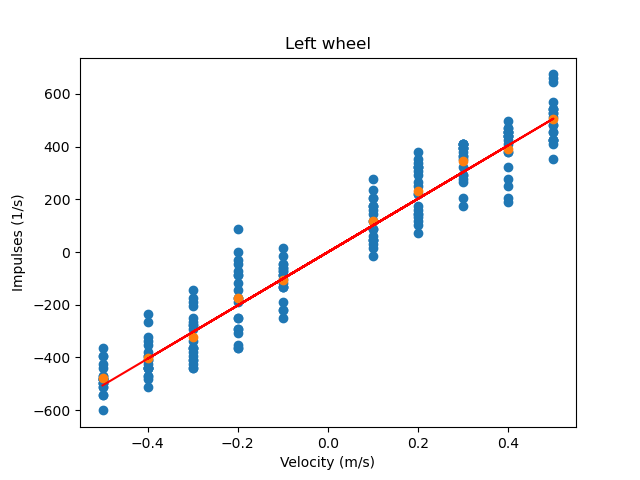
\includegraphics[width=\textwidth]{img/lw_nf.png}
	\end{subfigure}
	\hfill
	\begin{subfigure}{0.5\textwidth}
		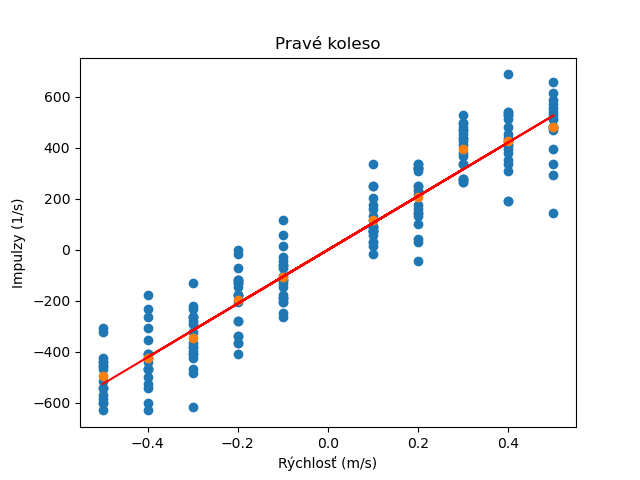
\includegraphics[width=\textwidth]{img/rw_nf.png}
	\end{subfigure}
	\caption{Získanie prevodu z~impulzov na~rýchlosť v~SI jednotkách.}
	\label{fig:rw_lw_nf}
\end{figure}

Ako prvú vec sme si vykreslili všetky \textbf{nazbierané dáta}. Tie sú zobrazené \textbf{modrou} farbou. Cez ne sme spravili \textbf{lineárnu regresiu}. Je zobrazená
ako \textbf{červená} úsečka. Z~nazbieraných dát sme si nakoniec spravili priemer, aby sme videli, ako presne aproximuje nami vypočítaná lineárna regresia priemer
nazbieraných dát. \textbf{Priemery} jednotlivých rýchlostí sú zobrazené ako \textbf{oranžové} body.

Môžeme si všimnúť, že~vypočítané priemery takmer presne ležia na~vypočítanej lineárnej regresii. Problémom je, ako už bolo spomenuté, že~dáta,
ktoré dostávame od robota sú veľmi zašumené. Preto z~nich nevieme priamo počítať polohu robota. Na zobrazenie veľkosti odchýlky sme spravili
meranie. Nechali sme robot aby prešiel dráhu štvorca so~stranou dlhou 1 meter a~rýchlosťou 0,5 \(\frac{m}{s}\). Výsledok bol veľmi nepresný.
Metrom sme si odmerali jeho \textit{x}-ovú a~\textit{y}-ovú súradnicu s~počiatkom v~bode, kde sme na~robote spustili náš ovládač. Jeho skutočná
poloha bola v~bode~(-0,3m,~0m). Čo~nám ale vypočítala odometriu je, že~sa robot nachádzal 4 metre od~počiatku súradnicového systému.

\subsection{Zisťovanie parametru \(\alpha\)}

Implementovali sme si preto dolnopriepustný kvadraticky filter. Fungovanie tohto filtra spočíva v~skombinovaní nového vstupného parametra a~starého parametra
uloženého vo~filtri v~danom pomere. Tento pomer je daný parametrom \textbf{alpha} $\alpha$.

$$ stavFiltra = \alpha * stavFiltra + (1 - \alpha) * nováVzorka $$

Jeho parameter \(\alpha\) sme získali viacerými meraniami. Začali sme najsilnejším filtrom s~hodnotou $\alpha$ rovnou  0,9.

\begin{figure}[!htbp]
	\begin{subfigure}{0.5\textwidth}
		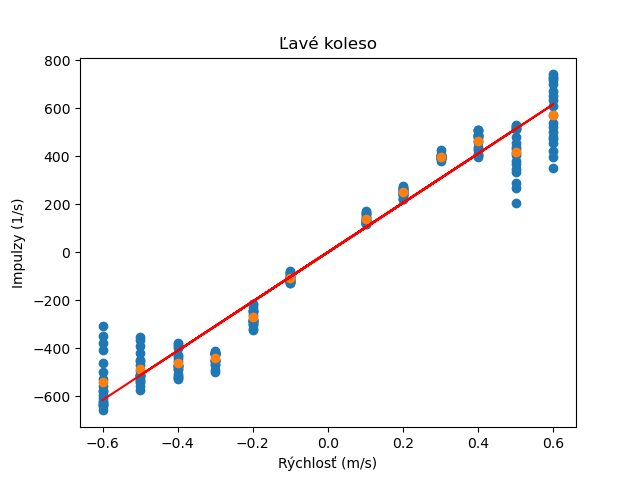
\includegraphics[width=\textwidth]{img/lw_09250.png}
	\end{subfigure}
	\hfill
	\begin{subfigure}{0.5\textwidth}
		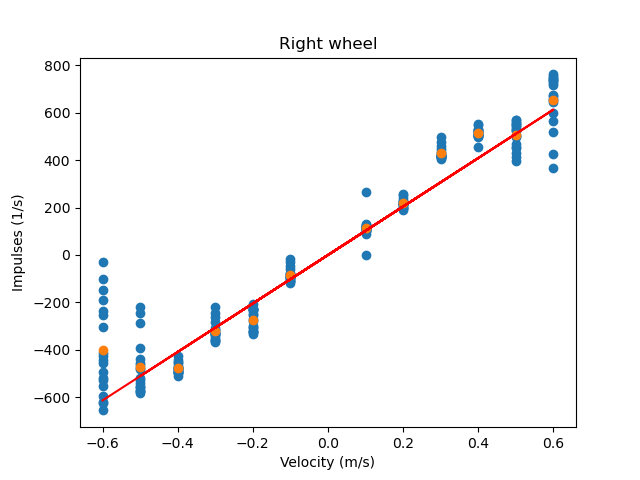
\includegraphics[width=\textwidth]{img/rw_09250.png}
	\end{subfigure}
	\caption{Získanie prevodu z~impulzov na~rýchlosť v~SI jednotkách. $\alpha$ = 0,9.}
	\label{fig:rw_lw_09250}
\end{figure}

Ako môžeme vidieť na~obrázkoch Obr.~\ref{fig:rw_lw_09250} a~Obr.~\ref{fig:rw_lw_nf} aplikácia filtra výrazne pomohla proti~šumu signálu.
Problémom pri~silnom filtri je to, že~ak na~začiatku merania dostaneme zlú hodnotu, tak~sa táto hodnota ťažko mení na~správnu. Tento
efekt si môžeme všimnúť skoro pri~každej meranej rýchlosti. Najviditeľnejší dopad môžeme vidieť pri~pravom kolese
na~Obr.~\ref{fig:rw_lw_09250} pri~rýchlosti -0,6$\frac{m}{s}$. Tento problém sme riešili postupným menením parametra filtru.
Aby sme predišli veľkému množstvu meraní, tak~sme použili metódy binárneho vyhľadávania. V~tomto prípade sme začali s~veľkou hodnotou
a~postupne sme skákali do~stredu nášho intervalu. Preto sme si ako ďalšiu hodnotu zvolili alphu $\alpha$ rovnú 0,7.

\begin{figure}[!htbp]
	\begin{subfigure}{0.5\textwidth}
		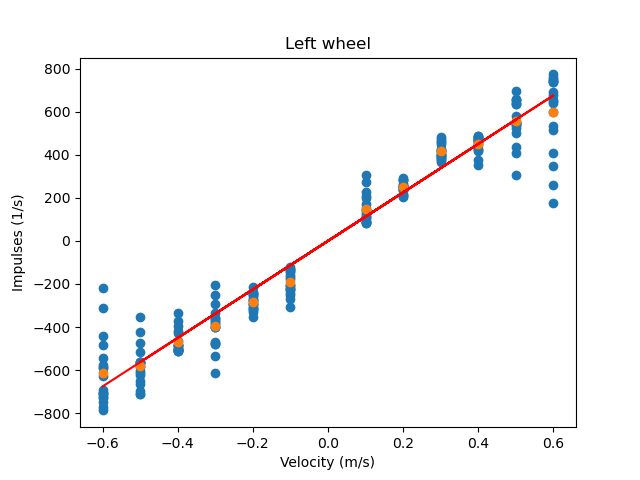
\includegraphics[width=\textwidth]{img/lw_07250.png}
	\end{subfigure}
	\hfill
	\begin{subfigure}{0.5\textwidth}
		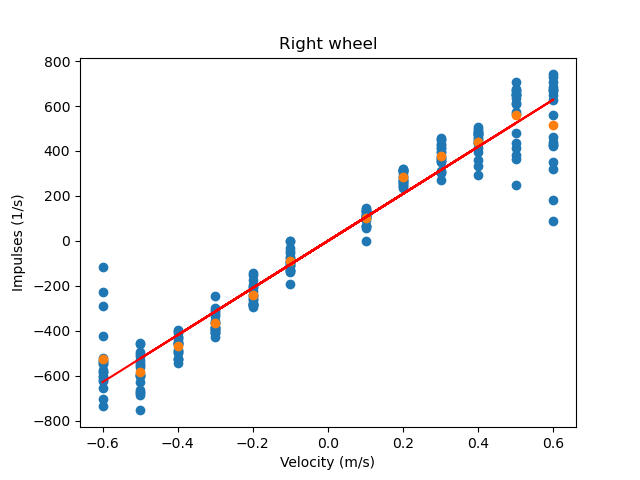
\includegraphics[width=\textwidth]{img/rw_07250.png}
	\end{subfigure}
	\caption{Získanie prevodu z~impulzov na~rýchlosť v~SI jednotkách. $\alpha$ = 0,7.}
	\label{fig:rw_lw_07250}
\end{figure}

Pri~použití hodnoty $\alpha$ rovnou 0,7 (Obr.~\ref{fig:rw_lw_07250}) sme zistili, že~sa hodnoty rýchlosti aj pri~aplikácii filtra výrazne menili. Ustálené
hodnoty zobrazené oranžovou farbou sú podobne ako pri~meraní s~filtrom s~alphou $\alpha$ rovnou 0,9 mimo lineárnej regresie.
Je to zapríčinené iným dôvodom ako pri~silnejšom filtri. Pokým pri~silnejšom filtri sme dostali zlú začiatočnú hodnotu, tak
už bolo zložité ju zmeniť. Pri~slabšom filtri, ak dostávame rozdielne vstupné hodnoty tak~sa výstupná hodnota filtra ľahko
mení. To má za dôsledok posun priemeru vstupných hodnôt. Tento efekt sa dá odstrániť zosilnením filtra, čiže zväčšením
koeficientu alpha $\alpha$. Spravili sme preto ďalšie meranie, kde sme použili hodnotu $\alpha$ rovnou 0,75.

\begin{figure}[!htbp]
	\begin{subfigure}{0.5\textwidth}
		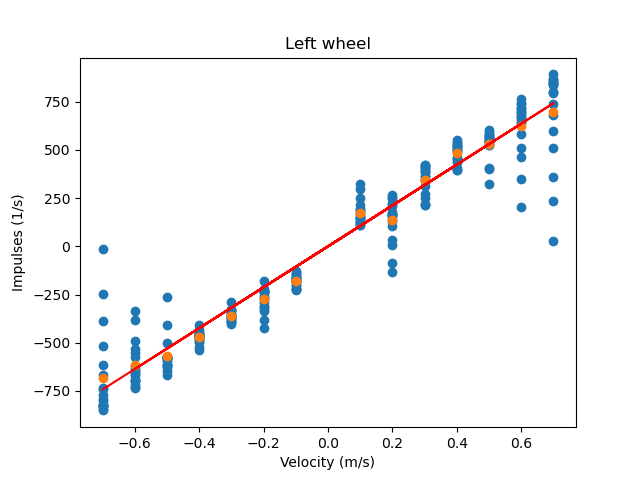
\includegraphics[width=\textwidth]{img/lw_075250.png}
	\end{subfigure}
	\hfill
	\begin{subfigure}{0.5\textwidth}
		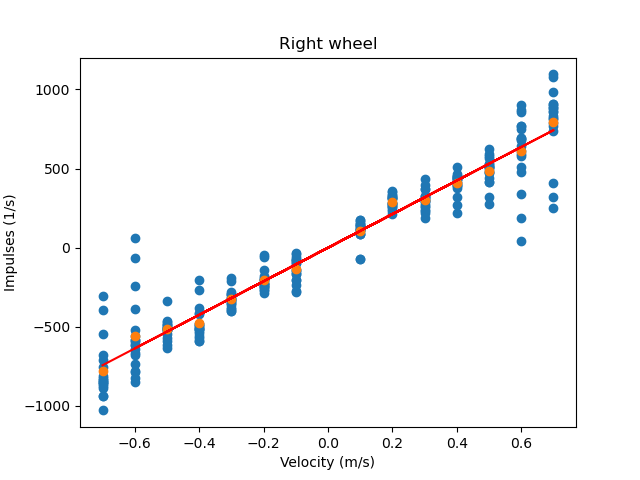
\includegraphics[width=\textwidth]{img/rw_075250.png}
	\end{subfigure}
	\caption{Získanie prevodu z~impulzov na~rýchlosť v~SI jednotkách. \(\alpha\) = 0,75.}
	\label{fig:rw_lw_075250}
\end{figure}

Obr.~\ref{fig:rw_lw_075250} zobrazuje graf výsledkov nameraných pri~aplikácii filtra s~koeficientom alpha o~veľkosti 0,75.
V~tomto prípade sa priemerné hodnoty na~rozdiel od~filtrov s~koeficientami alpha 0,9 a~0,7 dostali takmer priamo na~úsečku
lineárnej regresie prevodu z~impulzov za~sekundu na~metre za~sekundu. Použitie silnejšieho filtra síce pomohlo rýchlejšiemu
ustáleniu hodnoty, ale skúsili sme ešte silnejší filter s~hodnotou alpha $\alpha$ rovnou 0,8.

\begin{figure}[!htbp]
	\begin{subfigure}{0.5\textwidth}
		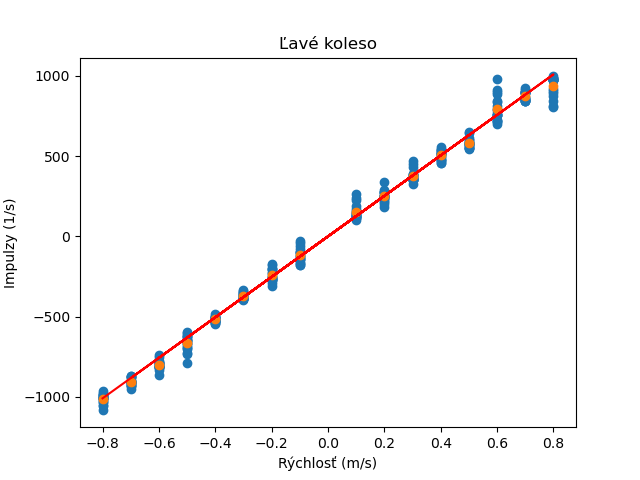
\includegraphics[width=\textwidth]{img/lw_08250.png}
	\end{subfigure}
	\hfill
	\begin{subfigure}{0.5\textwidth}
		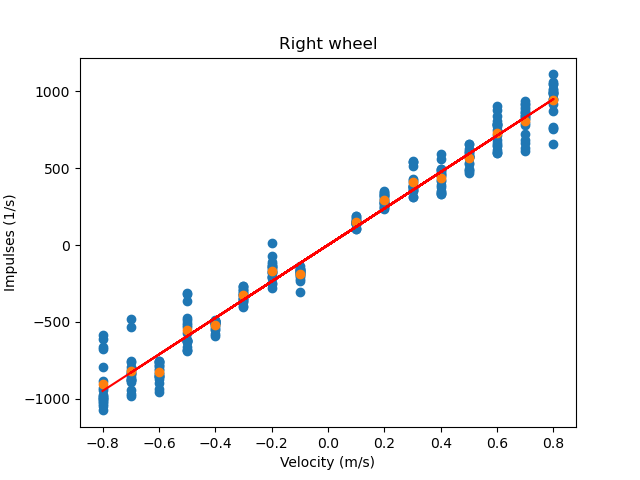
\includegraphics[width=\textwidth]{img/rw_08250.png}
	\end{subfigure}
	\caption{Získanie prevodu z~impulzov na~rýchlosť v~SI jednotkách. $\alpha$ = 0,8.}
	\label{fig:rw_lw_08250}
\end{figure}

Ako môžeme vidieť na~Obr.~\ref{fig:rw_lw_08250} ustálenie hodnôt je veľmi jednoznačné. Vybrali sme si preto filter s~hodnotou
koeficientu alpha $\alpha$ rovnou 0,8. Zatiaľ všetky dáta čo sme merali boli s~frekvenciou 4Hz (1 vzorka za 250 milisekúnd).
Pre~presnejší výsledok sme túto frekvenciu ešte zvýšili. Z~testov robota sme vypozorovali, že~najfrekventovaniejsia frekvencia,
ktorú môže robot sprostredkovať je 10Hz (1 vzorka za 100 milisekúnd). Spravili sme si preto test na~prevod rýchlosti ešte raz
s~rovnakou hodnotou koeficientu alpha $\alpha$ rovnou 0,8, ale s~frekvenciou 10Hz namiesto už spomenutých 4Hz.

\begin{figure}[!htbp]
	\begin{subfigure}{0.5\textwidth}
		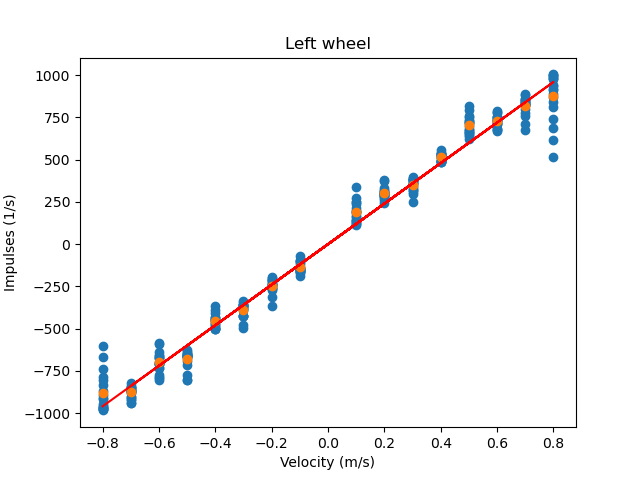
\includegraphics[width=\textwidth]{img/lw_08100.png}
	\end{subfigure}
	\hfill
	\begin{subfigure}{0.5\textwidth}
		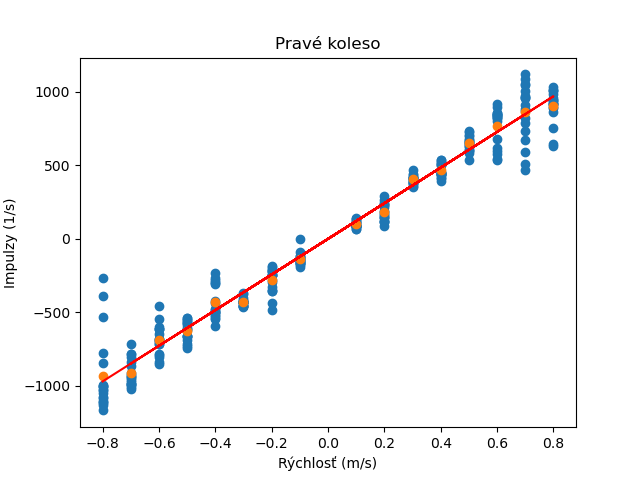
\includegraphics[width=\textwidth]{img/rw_08100.png}
	\end{subfigure}
	\caption{Získanie prevodu z~impulzov na~rýchlosť v~SI jednotkách. $\alpha$ = 0,8 a~frekvenciou 10Hz.}
	\label{fig:rw_lw_08100}
\end{figure}

Najlepšia možná hodnota tohto koeficientu nám vyšla $\alpha$ rovná 0,8. Pri~implementácii tohto filtra sme museli myslieť na~dôležitú vec.
Keď sa zmenia jednorazovo impulzy na~hodnotu 0 a~hneď spať, tak~nám táto vzorka pokazí výsledok. Musíme preto túto vzorku ignorovať. Ďalšia
prekážka, ktorú sme mali pred sebou bola zmena rýchlosti. Obyčajná implementácia filtra by nám spomalila zmenu vypočítanej rýchlosti
a~teda aj veľkú odchýlku v~polohe. Tento problém sme opravili prestavením počiatočnej hodnoty filtra na~prvú hodnotu po~zmene rýchlosti.
Toto riešenie sa ukázalo ako najlepšie so skúšaných riešení.

Problém so~zlou počiatočnou hodnotou môžeme vidieť aj na~posledom grafe Obr.~\ref{fig:rw_lw_08100}. Tento problém sme vyriešili
predpočítavaním prvej hodnoty filtra po~zmene rýchlosti. Keďže sme už mali koeficienty lineárnej regresie, tak~sme ich využili
na~predpočítanie počiatočnej hodnoty. Výsledok tohto postupu vidíme na~nasledujúcom grafe.

\begin{figure}[!htbp]
	\begin{subfigure}{0.5\textwidth}
		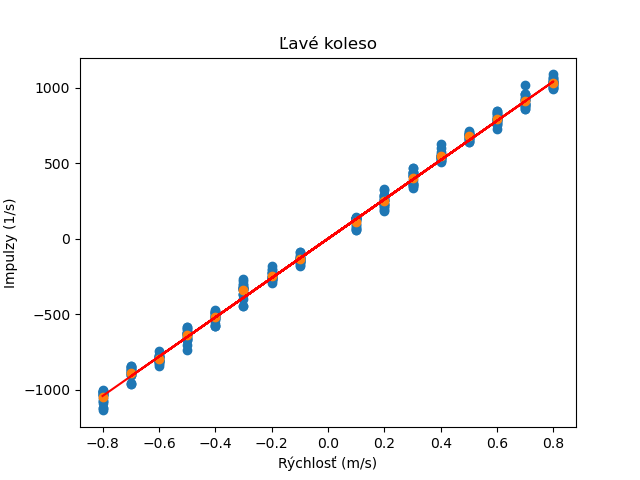
\includegraphics[width=\textwidth]{img/lw_08100_3.png}
	\end{subfigure}
	\hfill
	\begin{subfigure}{0.5\textwidth}
		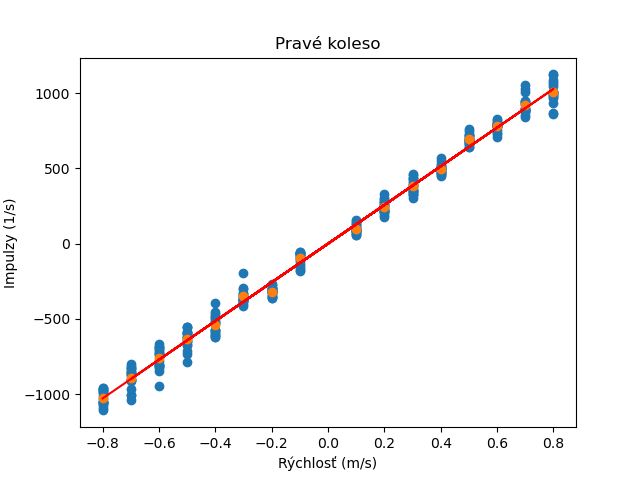
\includegraphics[width=\textwidth]{img/rw_08100_3.png}
	\end{subfigure}
	\caption{Získanie prevodu z~impulzov na~rýchlosť v~SI jednotkách. $\alpha$ = 0,8 a~frekvenciou 10Hz a~prvou prepočítanou hodnotou.}
	\label{fig:rw_lw_08100}
\end{figure}

